% Chapter 5

\chapter{Caso de uso}
% Write in your own chapter title
\label{Capitulo 5}
\lhead{Capítulo 5. \emph{Caso de uso}} % Write in your own chapter title to set the page header

Con el objetivo de poner a prueba la librería presentada, en este capítulo se  describe como extender una aplicación web desarrollada con continuations para que pueda adaptarse al contexto.

Se utiliza como punto de partida una aplicación web que se encuentra en el repositorio publico de Cincom$ ^{\textregistered}$ dentro de los ejemplos de Seaside, e implementa una tienda \emph{on line} que permite encargar sushi.

Antes de agregar la sensibilidad al contexto, se reemplazan el tipo de producto por otro que pueda ser identificado con un código de barra. En este caso, se utilizarán libros.

Además, se le realizan modificaciones a los componentes de Seaside para utilizar Scriptaculous y Meteoroid con el fin de reducir la transferencia de datos y mejorar la velocidad de refresco de cada actualización\cite{Fernandez09}.

A continuación se detalla el modelo de negocio de la aplicación web previo a agregar la extensión. Luego se detallan los componentes de Seaside (junto con los de Scriptaculous y Meteoroid) que posibilitan la utilización del modelo. Para finalizar, una vez descripta la aplicación web, se explica como expandirla para proporcionar adaptabilidad al contexto.


\section{El modelo de negocio de la aplicación web}

El modelo de negocios de la tienda de libros consiste en registrar todas las ventas realizadas (clase Order). De cada venta se conoce el conjunto de libros que se solicitaron, la dirección de facturación y de entrega de los libros, y los datos de la tarjeta de crédito desde donde se realizó el pago (ver Figura \ref{WAStoreModel}).

\begin{figure}[ht!]
\centering
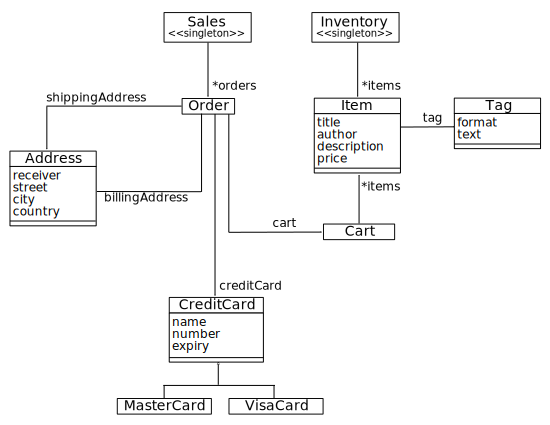
\includegraphics[scale=0.9]{UMLWAStoreModelClassDiagram}
\caption{Diagrama de clases UML del modelo de negocio de la tienda de libros}
\label{WAStoreModel}
\end{figure}

De cada libro (clase \emph{Item}) se conocen los atributos \emph{titulo}, \emph{autor/es}, \emph{descripción}, \emph{precio} y la \emph{descripción de un código de barras} (clase \emph{Tag}).

Las clases \emph{Sales} y \emph{Inventory} implementan el patrón de diseño \emph{Singleton}\cite{Gamma95}, y se encargan de almacenar las compras consumadas y los productos del inventario, respectivamente.


\section{La interfaz proporcionada por Seaside}

Para poder interactuar con el modelo existen un conjunto de componentes de Seaside, que dan forma a la aplicación web accesible por el usuario.

Mientras el usuario navega por la tienda on line, realiza consultas sobre el catálogo de productos (clase \emph{Inventory}, ver Figura \ref{bookstoreNetResultSequenceDiagram}). A su vez, puede agregar algún producto (clase \emph{Item}) a un carro de compras (clase \emph{Cart}), o sacarlo del carro de compras si es que ya no desea comprarlo (ver Figura \ref{bookstoreNetfillCartSequenceDiagram}).

\begin{figure}[ht!]
\centering
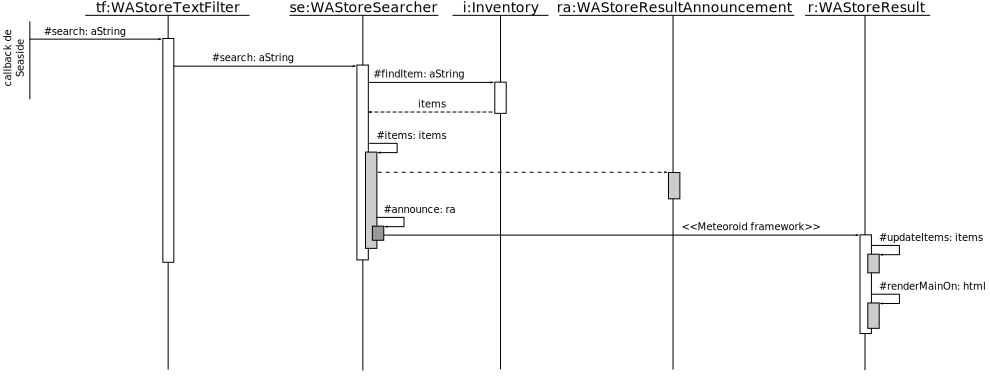
\includegraphics[scale=0.50]{bookstoreNetResultSeasideUMLSequenceDiagram}
\caption{Diagrama de secuencia UML de la búsqueda de productos}
\label{bookstoreNetResultSequenceDiagram}
\end{figure}

\begin{figure}[ht!]
\centering
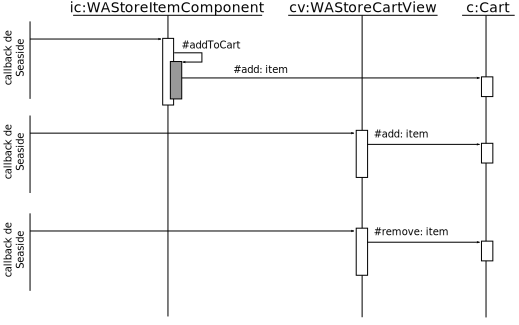
\includegraphics[scale=0.80]{bookstoreNetfillCartSeasideUMLSequenceDiagram}
\caption{Diagrama de secuencia UML de la carga de productos al carro de compras}
\label{bookstoreNetfillCartSequenceDiagram}
\end{figure}

Cuando el cliente desea hacer efectiva la compra, se le solicitan dos direcciones: una de envío del producto y otra para enviar la facturación (clase \emph{Address}). Para cada dirección deberá completar los atributos \emph{país}, \emph{ciudad}, \emph{calle} y \emph{nombre de la persona que recibirá} ya sea los libros o la facturación.

Por último, debe completar la información de su tarjeta de crédito (subclases de \emph{CreditCard}) y confirmar la compra. La confirmación de la compra significa la creación de una instancia de la clase \emph{Order} para registrar la compra. Esta instancia será automáticamente almacenada en la clase \emph{Sales} (ver Figura \ref{bookstoreNetSequenceDiagram}).

\begin{figure}[ht!]
\centering
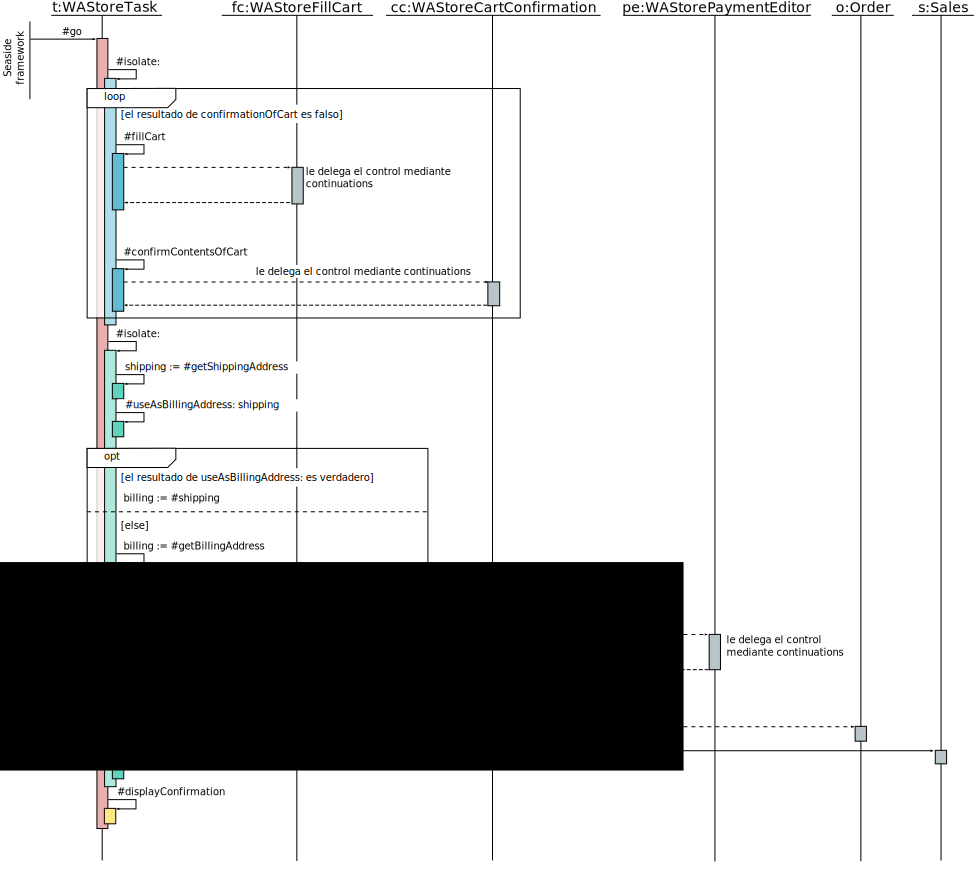
\includegraphics[scale=0.53]{bookstoreNetSeasideUMLSequenceDiagram}
\caption{Diagrama de secuencia UML de la tienda de libros}
\label{bookstoreNetSequenceDiagram}
\end{figure}

Es importante notar que en el método \emph{\#go} de la clase WAStoreTask se detalla el proceso completo, desde que el cliente se encuentra modificando el carro de compras, hasta que termina de abonar por la compra realizada. En esta descripción, se aíslan 2 subprocesos, la \emph{selección de los productos} y el \emph{pago}.

Una vez que se \emph{confirmó} la selección de los productos, el método \emph{\#isolate:} (perteneciente al framework Seaside) se encarga de descartar cualquier solicitud del navegador web que intente modificar el carro de compras. Lo mismo sucederá cuando se culmine de detallar la información de la tarjeta de crédito, bloqueando en este caso cualquier modificación de la orden generada.


\section{¿Cómo se utiliza la librería de adaptación al contexto?}

Si se extendiese el ejemplo presentado mencionando que la tienda de libros posee varios locales de venta al público en los que desea proveer un servicio adicional cuando un usuario (que se encuentra utilizando la aplicación web) accede. El servicio en cuestión, consiste en simplificar la búsqueda de la descripción y el precio de un articulo, a partir de la utilización de un código de barra.

El primer paso para proporcionar la sensibilidad al contexto es que el componente raíz de la aplicación web extienda a la clase \emph{MeteoroidNS.Meteoroid}.

Luego, es necesario agregar las librerías \emph{PhonegapLibrary}, \emph{ListenerEngineLibrary} y \emph{OSCLibrary} a la aplicación web. Por último se deberá agregar una variable de instancia para almacenar el componente \emph{MeteoroidNS.Listener}, que deberá ser \emph{renderizado} al final del método \emph{\#renderContentOn: html} del componente raíz.

A continuación para cumplir con los nuevos requisitos de la tienda de libros, se detallará el uso del sensor de posicionamiento para detectar que el usuario se encuentre dentro de un local de venta. Luego, se explicará el acelerómetro, el cual es necesario para detectar que el usuario desea escanear un código de barras. Y por ultimo, un \emph{sensor de códigos de barra} detectará si el código escaneado existe en el modelo de negocio.


\subsection{Sensor de posicionamiento}

Para detectar si el usuario se encuentra físicamente dentro de una tienda, es necesario establecer un polígono que delimite que posiciones pertenecen a una tienda. Luego, se utiliza a la librería para crear una \emph{Condition} que comprobará si la posición actual de un dispositivo se encuentra dentro de dicho polígono\footnote{Utilizando latitudes y longitudes como coordenadas.}. Por último, es necesario asociar esta condición a un \emph{trigger}, para que el servidor pueda coordinar la adaptación necesaria.

El código necesario para generar el trigger (ver Figura \ref{PositionInsideZoneExample}), primero crea a una instancia de la clase OSCPositionConditionBuilder al enviar el mensaje \emph{\#position} a la clase \emph{OSCConditionBuilder}.

\begin{figure}[ht!]
\begin{Verbatim}
insideTrigger := (OSCConditionBuilder position)
	inside: ((List new)
		add: -34.577301 @ -59.089359;
		add: -34.576801 @ -59.088829;
		add: -34.577690 @ -59.084999;
		add: -34.579041 @ -59.088242;
		add: -34.577793 @ -59.089119;
		add: -34.577339 @ -59.089279;
		add: -34.577301 @ -59.089359;
		yourself);
	callback: [self whenInside].
\end{Verbatim}
\caption{Código fuente para comprobar si una posición se encuentra en una zona}
\label{PositionInsideZoneExample}
\end{figure}

Como se desea conocer cuando el cliente ingresa a una tienda, se envía el método \emph{\#inside:} a la instancia del builder con una lista de posiciones como parámetro. Estas coordenadas determinan el perímetro de uno de los locales en particular (ver Figura \ref{satImageWithPolygon}).

\begin{figure}[ht!]
\centering
\includegraphics[scale=0.50]{satImageWithPolygon}
\caption{Mapa con el polígono en donde se encuentra la tienda}
\label{satImageWithPolygon}
\end{figure}

Luego, con el método \emph{\#callback:} se establece el comportamiento que debe realizar el servidor si el cliente \emph{dispara} ese \emph{trigger}. En este caso, enviará el mensaje \emph{\#whenInside} a la instancia que contenga la declaración anterior.

Dado que el trigger previo solo detecta cuando un usuario entra a una tienda, también es necesario controlar la condición opuesta para detectar cuando el cliente sale de la tienda, y en ese momento desactivar el servicio de búsquedas por código de barras

Lo único que será necesario cambiar será el método \emph{\#inside:} por \emph{\#outside:} (ver Figura \ref{PositionOutsideZoneExample}).

\begin{figure}[ht!]
\begin{Verbatim}
outsideTrigger := (OSCConditionBuilder position)
	outside: ((List new)
		add: -34.577301 @ -59.089359;
		add: -34.576801 @ -59.088829;
		add: -34.577690 @ -59.084999;
		add: -34.579041 @ -59.088242;
		add: -34.577793 @ -59.089119;
		add: -34.577339 @ -59.089279;
		add: -34.577301 @ -59.089359;
		yourself);
	callback: [self whenOutside].
\end{Verbatim}
\caption{Código fuente para comprobar si una posición se encuentra fuera de una zona}
\label{PositionOutsideZoneExample}
\end{figure}

A continuación, para que el servidor relacione a un trigger con un cliente en particular, es necesario solicitarle a una instancia de la clase \emph{Listener} (accesible desde la sesión de usuario de Seaside\footnote{Es importante destacar que todo el comportamiento de la sensibilidad al contexto se describe dentro de los \emph{WAComponent} de Seaside, y fuera del modelo de negocio.}) que lo \emph{recuerde} mediante el método \emph{\#remember:} (ver Figura \ref{PositionRememberListeningExample}).

\begin{figure}[ht!]
\begin{Verbatim}
self session listener remember: insideTrigger.
\end{Verbatim}
\caption{Código fuente para que un cliente sea sensible a un trigger.}
\label{PositionRememberListeningExample}
\end{figure}

Por el contrario, para que el navegador web deje de ser sensible a un \emph{trigger} deberá indicarle al \emph{listener} que lo \emph{olvide} utilizando el método \emph{\#forget:} (ver Figura \ref{PositionForgetListeningExample}).

\begin{figure}[ht!]
\begin{Verbatim}
self session listener forget: insideTrigger.
\end{Verbatim}
\caption{Código fuente para que un cliente deje de ser sensible a un trigger.}
\label{PositionForgetListeningExample}
\end{figure}

\subsection{Sensor de aceleración}

Luego de detectar la posición del usuario, si este se encuentra en una tienda es necesario reconocer si su intención es escanear un código de barras.

Para lograr esto, cuando se encuentra dentro de una tienda (el método \emph{\#whenInside}), se deberán registrar que posturas del dispositivo activarán la lectura de códigos de barra y en que posturas estas deberían desactivarse.

Por ejemplo, cuando el dispositivo se encuentra de forma vertical se asume que el usuario se encuentra en una postura ideal para utilizar la aplicación web. Por el contrario, cuando el usuario posiciona el dispositivo en forma apaisada, será interpretado como que el usuario desea leer un código de barras (ver Figura \ref{devicePostures}).

\begin{figure}[ht!]
\centering
\includegraphics[scale=0.50]{devicePostures}
\caption{Postura vertical y horizontal de un dispositivo}
\label{devicePostures}
\end{figure}

Al describir la postura de escaneo de códigos de barra se tiene en cuenta cierta movilidad o margen de error mostrado en la \emph{vista lateral}. Esta flexibilidad permitirá rotar hacia atrás el dispositivo cuando se encuentra en horizontal.

Luego, para definir la postura de escaneo es necesario utilizar 2 triggers, uno para cada tipo de apaisamiento. El primer trigger se encargará de detectar un angulo de 90 grados desde la posición vertical en sentido contrario a las agujas del reloj, mientras que segundo trigger se encargará de los 90 grados en sentido horario.

Teniendo en cuenta los extremos para cada una de las posturas se plantea como valores medios los puntos [x:7, y:0, z:5] y [x:-7, y:0, z:5] (ver Figura \ref{ScanBarcodePostureExample}). Luego el margen de error es para ambas posturas iguales [x:5, y:1, z:5]\footnote{Al eje del acelrómetro \emph{y} se le deja un margen de error de $\pm1$ $m/s^2$ para que el usuario pueda encontrar de forma sencilla la postura para escanear el código de barra, y no tenga que lidiar con la sensibilidad ofrecida por los acelerómetros de distintos dispositivos.}

\begin{figure}[ht!]
\begin{Verbatim}
scanningPosture1 := (OSCConditionBuilder acceleration)
	when: 7 @ (0 @ 5);
	acceptError: 5 @ (1 @ 5);
	callback: [self wantScanBarcodes].
scanningPosture2 := (OSCConditionBuilder acceleration)
	when: -7 @ (0 @ 5);
	acceptError: 5 @ (1 @ 5);
	callback: [self wantScanBarcodes].
\end{Verbatim}
\caption{Código fuente para describir la postura de escaneo de código de barras}
\label{ScanBarcodePostureExample}
\end{figure}

Nuevamente, es necesario recordar que habrá que informarle al \emph{Listener} de la sesión del usuario mediante el método \emph{\#remember:} si es que deseamos reconocer este entorno.

Por otra parte, se determina que el usuario quiere navegar por la aplicación web cuando no se encuentra en una postura de escaneo. Para identificar esto se define un trigger con una condición compleja (ver Figura \ref{NavigationPostureExample}).

\begin{figure}[ht!]
\begin{Verbatim}
navigationPosture := (OSCConditionBuilder complex)
	when: [:env |
		((env acceleration)
			whenNot: -7 @ (0 @ 5);
			acceptError: 5 @ (1 @ 5))
		&
		((env acceleration)
			whenNot: 7 @ (0 @ 5);
			acceptError: 5 @ (1 @ 5))];
	callback: [self wantNavigate].
\end{Verbatim}
\caption{Código fuente para describir la postura de escaneo de código de barras}
\label{NavigationPostureExample}
\end{figure}

Dentro del bloque de código que se le pasa como parámetro al método \emph{\#when:}, la variable \emph{env} permitirá acceder a la clase \emph{OSCConditionBuilder} dentro de la condición compleja. También es importante notar el método \emph{\#whenNot:} que niega la ocurrencia de esa condición. Por último, el operador \& (comúnmente llamado ``and'') permite la concatenación de condiciones para formar una más compleja.


\subsection{Sensor de códigos de barra}

En el momento que el \emph{acelerómetro} detecte que el usuario se encuentra en la postura adecuada para escanear un código de barra, la aplicación web deberá cargar en el dispositivo móvil del cliente los triggers adecuados para reconocer el código de barra de cada libro (ver Figura \ref{BarcodeTriggerExample}).

\begin{figure}[ht!]
\begin{Verbatim}
bookTriggers := OrderedCollection new.
Inventory default allItems do: [:item | 
	bookTriggers add: ((OSCConditionBuilder tag)
		when: item tag format | item tag text;
		callback: [ self findTaggedWith: item tag ])]
\end{Verbatim}
\caption{Código fuente para describir las condiciones relacionadas con códigos de barras aceptados por el modelo}
\label{BarcodeTriggerExample}
\end{figure}

En este caso se agregan todos los triggers a una colección de objetos, notar que en el método \emph{\#when:} se envía como parámetro el \emph{formato} del código y el \emph{texto} que simboliza la secuencia de caracteres o dígitos del código.

Para finalizar será necesario solicitarle al \emph{Listener} de la sesión del usuario que recuerde cada uno de los triggers contenidos en la colección \emph{bookTriggers}, para que el navegador pueda utilizarlos para reconocer entornos\footnote{Del lado del cliente, el navegador solo mostrará la pantalla de escaneo de códigos de barras si es que existe alguna condición dentro del \emph{listener} de códigos de barras.}.

Como consecuencia del proceso anterior, si el cliente enfoca la cámara de su dispositivo hacia el código de barras de un libro, el navegador web procederá a mostrar la información relacionada con dicho libro.

Cabe señalar que así como se describieron estos sensores, necesarios para desarrollar el caso de uso planteado, existen otros (como el estado de la batería, el tipo de conexión a internet, la orientación con respecto al Polo Norte, etc.) que también pueden ser utilizados. Además, si la situación lo requiere, se pueden crear una gran cantidad de nuevos sensores que ayuden a reconocer las necesidades del usuario.